% !TeX root = ../main.tex
% Add the above to each chapter to make compiling the PDF easier in some editors.

\chapter{Optimization}\label{chapter:Optimisaiton}

In this chapter is the main contribution of this thesis. We will look at 3 different optimizations

\section{Unit conversion}\label{section:conversion}
The application could previously only work on "gram", "ml" aswell as a item count. Recipies commonly feature units like tablespoons(tbsp), teaspoon(tsp), dashes, pinches, and in the US a lot of ingredients are measured in "cups". This system is based on volumes, unlike the usual metric approach where most measurements are made in mass. To provide a universal usability we have also included imperial aswell as us-customary units. While we can not convert between the us customary system and regular imperial system, we implemented a converter for both systems to the metric scale. The systems can be changed in the configuration of the application. Because we are using a meal plan provided by the austrailian government, the default system is set to imperial. All operable units are listed in table *insert table*. \\

%todo: Describe implementation

\begin{table}[htpb]
  \centering
  \begin{tabular}{|l|l|l||l|l|l|}
  	\hline
  	Name & Symbol & SI factor & Name & Symbol & SI factor \\
  	\hline
    \multicolumn{3}{|c|}{Imperial}
    \multicolumn{3}{|c|}{ US-Customary}
    \hline
    \multicolumn{6}{|c|}{Volume}
    \hline
  \end{tabular}
  \caption[Covered units]{Units covered by the program}\label{table:units}
\end{table}

There are a couple of problems within the system of units that not covered by our algorithm. Some measurements, like the "pinch", are not even clearly defined within one system. Sticking with our example, the "pinch": a pinch is historically defined as "the amount that can be taken between the thumb and the forefinger" \cite{rowlett2000dictionary}. Obviously this "measurement" varies significantly person to persons. To provide more consistent means to quantify a pinch in the US a pinch is defined as 1/16th of a taespoon, while in the UK it is defined as 0.355625g. This leaves us with a unit that can represent both mass and volume, without regard for density. This makes the "pinch" and similar inconsistent measurements unfitting for a scientific approach to a healthy diet. Our application features prestored recipies. These recipes contain the informaton for quantities aswell as units for each ingredient. This combination of user configurated unit interpretation and prestored, context-free, inconsistent units may lead to a deviation of the optimal nutrition levels defined by the mealplan.
The combination of count, volume and mass units leads us to another problem not covered by our unit converter. The converter only converts within the context of mass or volume, but does not feature conversion between them. This may lead to the final shopping list containing entries for each type. Integrating a database with densities and average mass for food items should fix this problem.


\section{Ingredient preprocessing}\label{section:preprocessing}
One problem of the initial application is that there are multiple occurences of the same ingredient, with a different suffix. For example the application might generate a list entry for "red onions" aswell as "red onions, thinly sliced". Simply dropping the suffix on the ingredients could help in some cases, like our onions, while for other cases droppign the suffix could be problematic. For "fried shallots" or "dried tomatoes" buying the product referenced in the recipe could save the user significant amounts of time, depending on the required procedure. In this section we will show, how we used data preprocessing to approach this problem.
Our preprocesser is regular expression based. Given our context, the possible input strings are already quite well defined. As we do not need to fulfill complex functionality, state of the art maschine learning approaches seem a bit far fetched. We feel that regular expressions provide enough functionality to solve our problems.

\begin{figure}
	\centering
	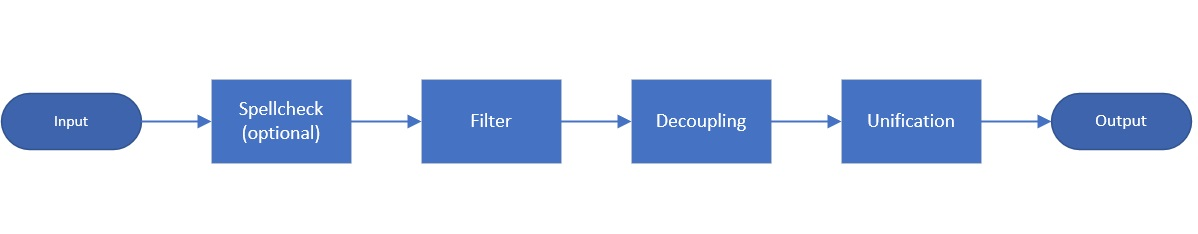
\includegraphics[scale=0.45]{Figures/pipeline.jpg}
	\caption[Preprocessing Pipeline]{Preprocessing Pipeline}\label{fig:pipe}
\end{figure}

Figure \ref{fig:pipe} shows how the individual ingredient names are preprocessed.
First we apply spellchecking, then we filter unnecessary information from the string. Followed by  decoupling for any String containing "and", finally we unify the format and spelling of the strings. In this section we will describe each step of our preprocessing pipeline in detail chronlogicaly.

\subsection{Spellchecking}\label{sub:spellcheck}
Before we can start processing the data, we need to make sure, our input is spelled correctly. Covering typos in regexes can be quite difficult and can also lowers readability of code. To get rid off any typos we use the pyspellchecker library \cite{spellchecker}. The spellechecker uses levenshtein Distance to find permutations within a frequency list. The spellchecker introduces a large performance overhead, which lead us to implement a configuration option "use\underline{•}spellchecker". This option allows the user to disable the spellchecker, if needed. Taking into account, that most people need to spend time reachign their local grocery market, the overhead should not be relevant in a "rolled out" application. Alternatively the spellcheck could be applied when adding new recipes to the database. This would reduce the impact to the performance of our programm significantly, since it only impacts our setup, but does not affect the program at runtime. Also we can assume that recipes are getting read multiple times, while we only need to write them once, further increasing the benefits of applying spellchecking while adding recipes.
\subsection{Filter}\label{sub:filter}
Recipes usually do not specify the requierd ingredients in their natural form. Ingredients are often already processed, for example vegetables are usually cut into smaller pieces or peeled in order to provide lower cooking times, a more pleasent texture or a more appealing look. For the grocery list these specifications do not matter. Only in few cases the product, aimed to be bought at the store is affected by the additional information contained in the recipes desciption. One example for this could be "dried" fruits or vegetables, as the preparation time would exeed the time a regular person is willing to invest into their daily meals.\\
In the filtering step, our preprocesser aims to eliminate irrelevant information. 
There are three different types of information we try to eliminate: 
\begin{itemize}
	\item Descriptions of cooking procedures(e.g cleaned, sliced, crushed),
	\item adjectives that further specify the procedures(e.g. "thinly","roughly"),
	\item "fancy" product descriptions like "crisp salad" or "fresh tomatoes"	
\end{itemize}
The first and the last point are handled with an identical approach. We use string matching for regular expressions and substitute any found pattern with an empty string. The pattern we are searching for are wordbound occurences of predefined strings. These strings are then combined in a disjunctive expression.
The list of words contained in our filter is read from the config.
The core reason to split up the list into two parts was to enhance readability and maintainability of the lists.\\
To filter adjectives that further describe our input, we simply search for any word ending in "ly". To avoid falsely eliminating food items like "jelly" we also integrated a list exceptions in our config.

The final step in our filter is the elimination of redundant commata, spaces or "and"s. To do this we simply match any occurance in the beginning or end of our input, aswell as any surplus spaces or commas within.
\subsection{Decoupling}\label{sub:decoupling}
Some ingredient descriptions feature a combination of multiple ingredients. To raise readability of our grocery list we try to decouple such items into a list of their components. For example, instead of having an item called "Salt and Pepper", we would prefer to split the item up into an entry for "salt" and another one for "pepper". For listings we have found that the usual format is having a leading generic term, followed by an instance. If lets say a recipe requires two different oils the item would be listed as: "oil, pumpkin seed and  apple". To split the input in its components, we use this function:
\begin{lstlisting}[language=python]
def decouple(input):
    pattern_and = re.compile(
        r"([\w\s]+,? )?([\w\s]+,? )?([\w\s]+,? )?([\w\s]+,?)?(and )([\w\s]+)"
    )
    match = pattern_and.match(input)
    components = []
    if match is None:
        return [input]
    if match.group(1) is not None:
        components.append(match.group(1))
    if match.group(2) is not None:
        components.append(match.group(2))
    if match.group(3) is not None:
        components.append(match.group(3))
    if match.group(4) is not None:
        components.append(match.group(4))
    if match.group(6) is not None:
        components.append(match.group(6))
    if components.__len__() > 2:
        head = components.pop(0)
        i = 0
        while i < len(components):
            components[i] = head + components[i]
            i = i + 1
    return components
\end{lstlisting}
The pattern seraches for any string containg "and " and groups text segments seperated by ",". If we can not match a "and"-pattern we return a list only containing our input. Otherwise we append every non empty group. Group 5 represents the "and " we are trying to eliminate and is conseqently not added.
Furthermore if we have more than 2 components we pop the head of the list, and add it to every remaining component. Sticking to our earlier example, the function would transform "oil, pumpkin and apple" into ["oil, pumpkin", "oil, apple"].
The programm assumes even distribution over each component. So the quantity defined by the recipe is devided by the number of components.

Furthermore we differenciate between the word "and" and the ampersand(and symbol) "\& ". The ampersand is used to describe flavours of ingredients. We must maintain any descriptions containing an "\& " symbol as splitting up here would result in a false result. 
\subsection{Unification}\label{sub:unify}
At this point, our initial input has been spellchecked, most irrelevant information should be filterd, and the input has been decomposed into elemental items.
As a last step, we need to make sure that any difference in spelling, wording and formating must be eliminated.
To unify the remaining inputs we try to substitute any possible option into one predefined one. We split the unification process into four parts.\\\\
First we try to unify any terms, or generalize terms.
There are a lot of possible wording options for terms like "fat-free" "gluten-free" and so on. Also there are product descriptions we can neglect. Brand loyalty is a the main factor in choosing products\cite{doi:10.1080/02642069600000006}. Consequently we assume that a customer would buy his regular brand of olive oil regardless of our  generated list specifying an extra-vergine olive oil or a regular one.
\begin{lstlisting}[language = python]
    item = re.sub(r"fat[ -]?free|non[ -]?fat", "fat-free", item)
	item = re.sub(r"(extra vergine )?olive oil", "olive oil", item)
\end{lstlisting}
The two examples of suppstitutions show how we can easily unify different spellings, with the first attribute describing a pattern and the second one its replacement on the stringe defined by the third attribute.
One generalisation not covered by our unification function, are requests for specific brands. While we can filter out upc-codes, brand names and their specific product descriptions require a much more complicated nlp system. For a single market and a fixed inventory list, this could be done by a filter similar to the one we described in (\ref{sub:filter}), covering amount of global brands and number of their products with a word filter is infeasible.\\\\
As mentioned earlier we also need to unify spelling. While our spellchecker (\ref{sub:spellcheck}) should cover any typos, there are still some words with multiple correct spelling options. In the word "yoghurt" the "h" is common for most english speaking countries, excluding canada and the united states. Our unification function covers common food items with multiple spelling options and substitutes them in a identical fashion as the earlier examples.\\\\
At this point there are only two tasks left. The mapping of words in singular and plural and the unification of the format.
To enhance readability and to unify the format we chose the to start with descriptions and end with the item name. To do that we invert the order of our string, at the first occurence of a comma.
\begin{lstlisting}
	pattern_unified_format = re.compile(r"([\w ]+), ([\w ]+)")
    match = pattern_unified_format.match(item)
    if match is not None:
        item = match.group(2) + " " + match.group(1)
\end{lstlisting} 
For handling singular and plural, we simply try to match strings with standard plural endings. We match while searching our grocery list for similar ingredients, and for any match of a singular and plural of the same word the plural word is written into the list. 

\section{Categorisaton}\label{section:categorisation}
The optimization of categorization is done by processing the input with the in \ref{section:preprocessing} mentioned preprocessor. 
The following chapter focuses on evaluating the categorisation aswell as grocery shopping list generation. We will compare our implementation with the inital implementation by asela \

